\chapter{Test Driven Development}
\label{chap:2_tdd}
\section{Overview on software testing}
Software testing is an essential part of the development process and lifecycle of a system, as it helps to verify that the implemented solution is reliable and performs as intended in most situations. Testing can be defined as the process of finding differences between the expected behavior specified by the system's requirements and models, and the observed behavior of the implemented software; unfortunately, it is impossible to completely test a non-trivial system. First, testing is not decidable; second, its activities must be performed under time and budget constraints \cite{OOSE}, therefore testing every possible configuration of the parameters of a system is unfeasible and impractical.
Today, developers often compromise on testing activities by identifying only a critical subset of features to be tested.

There are many approaches to software testing, each having has its own goals and methods, as well as a different suite of tools built to support them and ensure that the testing process is always consistent, its execution is easily automated, and the test outcomes are always clear; furthermore, different techniques are often used in combination with each other to guarantee that a software product is thoroughly tested and conform to its specification. 
More in detail, the main testing techniques are: 
\begin{itemize}
    \item \textbf{Unit Testing}: a method of testing individual units or components of a software product in isolation; its goal is to verify that each of these units is working correctly and meets its expected behavior. These kinds of tests are usually written by the developers who also wrote the corresponding production code, and they are run automatically as part of the build process. Techniques also exist to generate input configuration for unit test automatically, by intelligently searching among the input space for the program.
    \item \textbf{Integration Testing}: two or more modules of an application are logically grouped together and tested as a whole. The focus of this type of testing is to find the defect on interface, communication, and data flow among modules. The top-down or bottom-up approach is used while integrating modules into the whole system.
    \item \textbf{System Testing}: a method of testing a complete software product against the specified requirements; can involve different activities, such as end-to-end testing - where it is ensured that the software meets the expected flow of operations when running in a real-world environment, on different hardware combinations, operating systems or web browsers, and with different input configurations - or smoke testing, where the goal is to verify that basic and critical functionality of the system under test is working fine at a very high level.
    \item \textbf{Acceptance Testing}: a method of testing a software product to ensure that it complies with the needs and expectations of the end user. The goal here is to verify that the software is fit for its intended purpose and that it meets the requirements of the user. Acceptance tests are often written by the end user or a representative of the end user.
    \item \textbf{Performance Testing}: one type of non-functional testing technique. It revolves around the process of evaluating a system's performance in terms of responsiveness and stability under a particular workload; it is usually done to determine how a system behaves in terms of various inputs and how it responds to different levels of traffic. Used to test availability, reliability, and other parameters.
    \item \textbf{Penetration Testing}: a kind of security testing, where a system, network, or application is exercised with the objective of identifying vulnerabilities that an attacker could exploit; this evaluation happens by simulating an attack and identifying any weaknesses that could be exploited by a malicious party. Penetration testing can be conducted by both internal and external security teams and is often used as a means to identify and remediate any potential security risks.
\end{itemize}



\subsection{Software Development Lifecycle}
Before discussing how testing activities are performed in more detail, it is essential to introduced how testing is integrated in the development process. The term Software Development Lifecycle (SDLC) refers to the entire process of developing and maintaining software systems, from the initial concept, to its end-of-life period; one of the first SDLC models introduced in software engineering is the Waterfall model; it is a linear, sequential approach to software development in which there is a strict, marked division between the different phases, such as requirements gathering, design, implementation, testing, and maintenance. While it has been employed for long, especially in monolithic applications, it has a few weaknesses, most notably not allowing for much iteration or flexibility during the development process: once a phase is completed, it is difficult to go back and make changes to earlier phases. This can lead to a very long feedback cycle between requirements specification and system testing, resulting in wasted time and resources in case a design flaw is not discovered until later in the development process. Additionally, the Waterfall model assumes that all requirements can be fully gathered and understood at the beginning of the project; such a simplification is often not applicable in modern software development, where ever-evolving requirements and functionalities are the norm. 
Finally, the model does not account for the fact that testing and deployment are ongoing processes, not a single event at the end of the project.
Figure \ref{waterfall_model} highlights the main phases of the Waterfall model.

\begin{figure}[H]
    \centering
    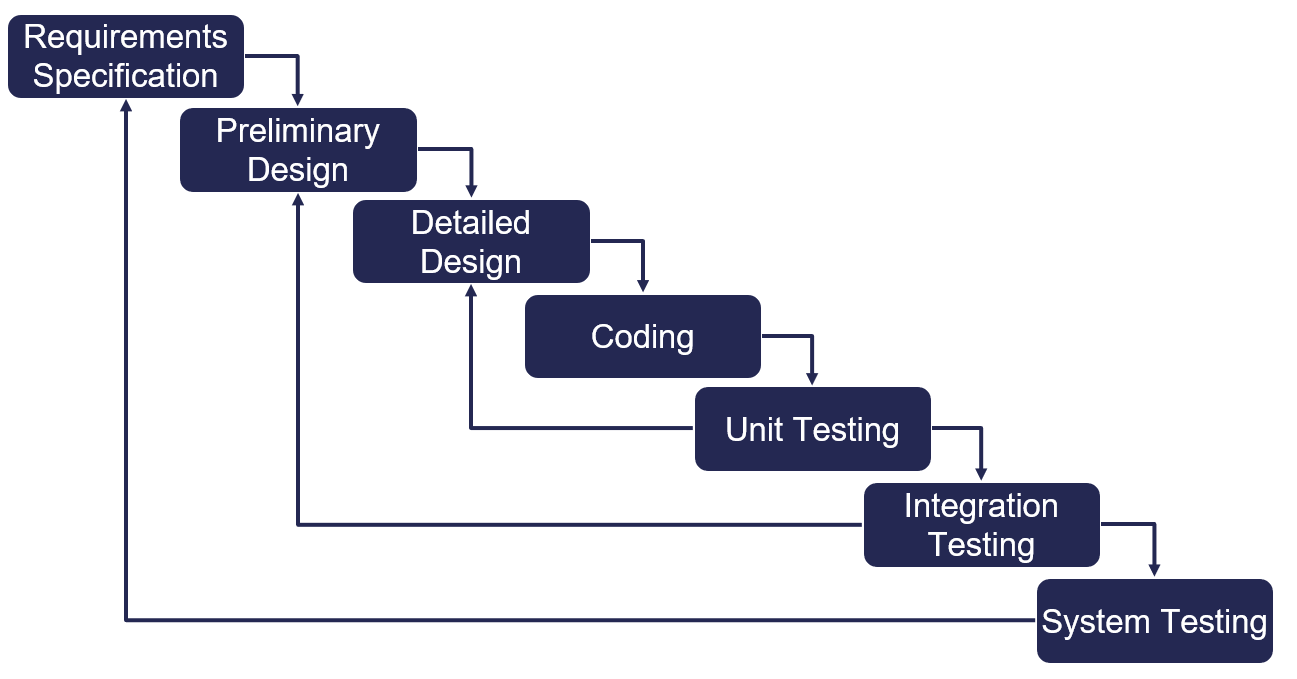
\includegraphics[width=10cm, scale=0.5]{figures/waterfall_model.png}
    \caption{The Waterfall model.}
    \label{waterfall_model}
\end{figure}

Modern software development strays away from non-incremental models, as today's applications are continuously evolving and adapting; instead, iterative approaches are preferred, where the sequential chain of the Waterfall model is replaced by a cyclical process during which the development team goes through multiple iterations or cycles of planning, designing, building, testing, and evaluating the product.

A key example is the Agile SDLC model, which values flexibility and collaboration, and prioritizes customer satisfaction and working software over strict plans and documentation. One of the main principles of Agile development is the use of small, cross-functional teams that work together to deliver working software in short iterations, or "sprints": this allows for frequent feedback and adjustments to be made throughout the development process between the clients and the development teams, rather than waiting until the end of a project to make changes.
Figure \ref{agile_model} highlights the phases of the Agile process:

\begin{figure}[h]
    \centering
    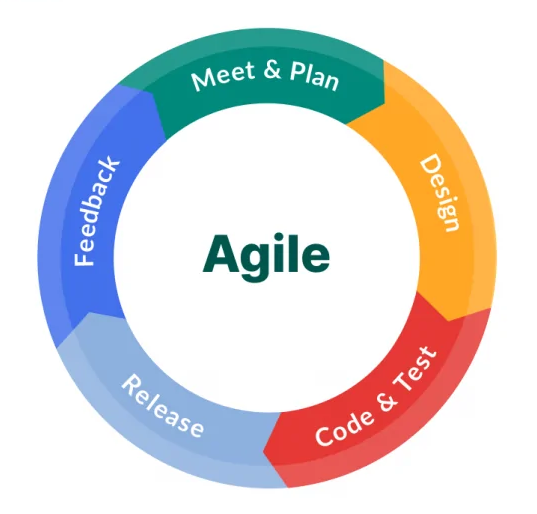
\includegraphics[width=8cm, scale=0.2]{figures/agile_model.jpg}
    \caption{The Agile model.}
    \label{agile_model}
\end{figure}

\noindent The main steps performed during each of these phases are summarized below:
\begin{itemize}
    \item \textbf{Design}: in this phase, the team designs the architecture, user interface and overall functionality of the software; the design process is iterative and collaborative, with the team working closely with customers, as well as with the stakeholders, with the objective to ensure that the software meets the agreed-upon needs.
    \item \textbf{Code \& Test}: in this phase, the team writes the code for the software and performs testing to ensure that it is functioning correctly; agile development places a strong emphasis on automated testing, which allows for quick feedback on the quality of the delivered code modules.
    \item \textbf{Release}: the team releases the software to customers and stakeholders; this allows developers to gather feedback on the software before the final release.
    \item \textbf{Feedback}: the team reviews the feedback received from customers and stakeholders and makes any necessary changes to the software. Since this feedback is also incorporated into the development process in an iterative manner, it allows the software to continuously improve over time.
    \item \textbf{Meet \& Plan}: the team meets to plan the next iteration of development, reviews the progress made in the previous iteration, sets goals for the next iteration, and assigns tasks to team members. The team also reviews and adjusts the development plan as needed to ensure that the software is on track to meet the customers' needs.
\end{itemize}



\section{Test-Driven Development}
\subsection{Overview}
Unit testing is arguably the most practiced testing technique, since by itself it can already provide a general assessment of the quality and reliability of a software solution. \tdd is a software development approach that builds on top of the concept of unit testing, firstly introduced in 2003 by Kent Back in the book "Test-Driven Development By Example" \cite{TDDByExample}; while there is no formal definition of the process, the goal is to "write clean code that works", as the author states. With \tdd, test cases are written before any production code is written: these tests are used to define the requirements for the system and to guide the development process, with 
the objective of this practice being for all these tests to pass before the development is complete, by continuously running the entire test suite as more features are tested and built; this can help to ensure the quality and reliability of software. Moreover, \tdd encourages software developers to write small, isolated units of code that are easy to test, maintain and understand, and will ultimately act themselves as a form of documentation for the developers. 
Compared to traditional testing and SDLC approaches, \tdd is an extremely short, incremental, and repetitive process, which make it strongly related to test-first programming concepts in Agile development and Extreme Programming; this advocates for frequent updates/releases for the software, in short cycles, while encouraging code reviews, unit testing and incremental addition of features.


At its core, \tdd is made up of three iterative phases: "\textit{Red}", "\textit{Green}" and "\textit{Blue}" (or "\textit{Refactor}"):
\begin{itemize}
    \item In the \textbf{\textit{Red}} phase, a test case is written for the chunk of functionality to be implemented; since the corresponding logic does not exist yet, the test will obviously fail, with the source code often not even compiling.
    \item In the \textbf{\textit{Green}} phase, only the code that is strictly required to make the test pass is written.
    \item Finally, in the \textbf{\textit{Blue}} phase, the implemented code, as well as the respective test cases, is refactored and improved. It is important to perform regression testing after the refactoring to ensure that the changes didn't result in any unexpected behaviors in other components.
\end{itemize}
Each new unit of code requires a repetition of this cycle \cite{GuidelinesTDD}. Figure \ref{tdd-cycle} provides a visual representation of the \tdd process:

\begin{figure}[h]
    \centering
    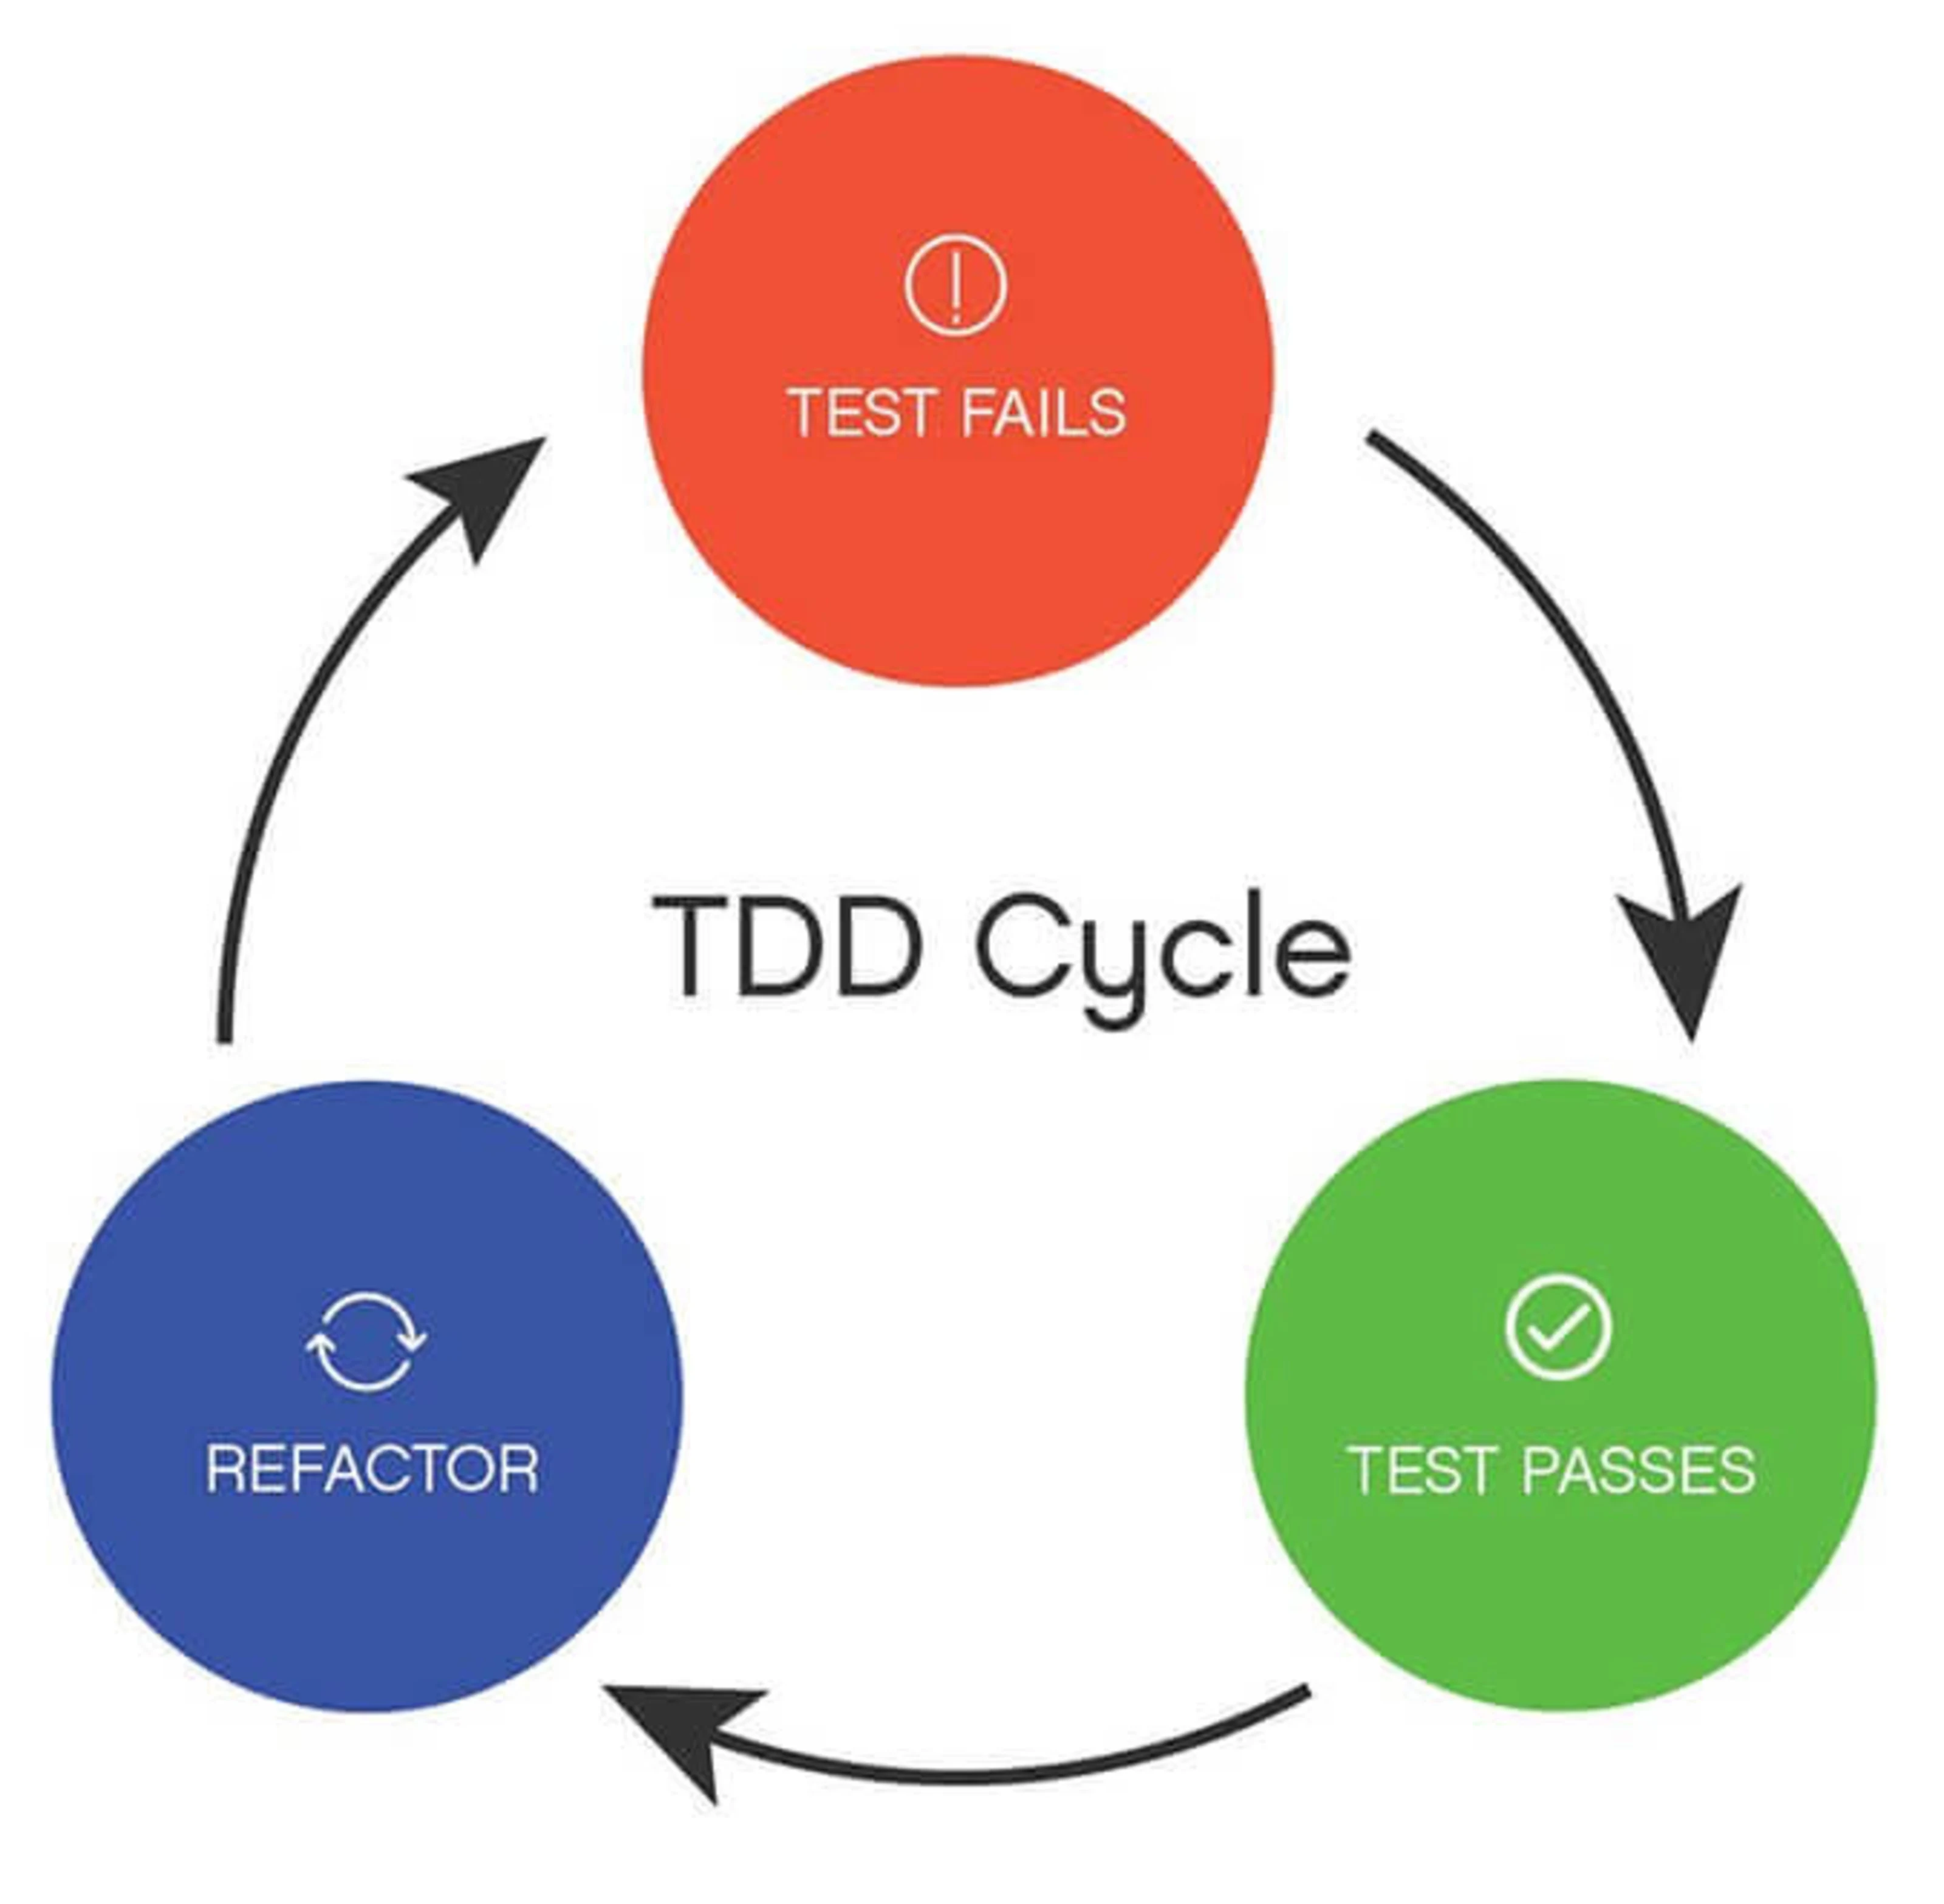
\includegraphics[width=8cm, scale=0.2]{figures/tdd_cycle.jpg}
    \caption{The Test-Driven Development cycle.}
    \label{tdd-cycle}
\end{figure}

As previously stated, each \tdd iteration should be extremely short, usually spanning from 10 to 15 minutes at most: this is possible thanks to a meticulous decomposition of the system's requirements into a set of User Stories, each detailing a small chunk of a functionality specified in the requirements; these stories can then be prioritized and scheduled to achieve an iterative implementation of the system. The specification of user stories can also vary in granularity: when using a fine-grained structure to describe a task, this can be broken up into a set of sub-tasks, each corresponding to a small feature; on the other hand, with coarser-grained tasks, this division is less pronounced \cite{DBLP:journals/tse/KaracTJ21}. Even when the same task is considered, the outcome of the \tdd process will change depending on the level of granularity employed when describing it; there is no overall right or wrong approach, rather it is something that comes from the experience of the developer to break tasks into small work items \cite{DBLP:journals/tse/KaracTJ21}.


\subsection{\tdd advantages and challenges}
The employment of \tdd can result in a series of benefits during the development process, such as:
\begin{itemize}
    \item \textbf{Very high code coverage}: coverage is a metric used to determine how much of the code is being tested; it can be expressed according to different criteria such as statement coverage - \ie how many statements in the code are reached by the test cases - branch coverage - \ie how many conditional branches are executed during testing - or function coverage - \ie how many functions are executed when running the test suite. While different coverage criteria result in different benefits, by employing \tdd we ensure that any segment of code written has at least one associated test case.
    \item \textbf{Improved code quality and maintainability}: as we are specifically writing code to pass the tests in place, and refactoring it after the "\textit{Green}" phase, we ensure that the code is cleaner and overall more optimized, without any extra pieces of functionalities that may not be needed, leading to a more maintainable architecture in the long run.
    \item \textbf{Regression testing}: by incrementally building a test suite as the different iterations of \tdd are performed, we allow the system to always be ready for this suite to run whenever new changes or functionalities are pushed to its codebase.
    \item \textbf{Improved code readability and documentation}: well-written tests serve as documentation for the code, making it easier for new contributors to understand it.
    \item \textbf{Simplified debugging and early fault detection}: whenever a test fails it becomes obvious which component has caused the fault: by adopting this incremental approach and performing regression testing, if a test fail we will be certain that the newly written code will be responsible. For this reason, faults are detected extremely early during the testing process, rather than potentially remaining hidden until the whole test suite has been built and executed.
\end{itemize}
Similarly, however, the \tdd approach can result in a series of pitfalls and challenges:
\begin{itemize}
    \item \textbf{Learning curve}: \tdd requires a different way of thinking about software development, which can be challenging for some developers to learn.
    \item \textbf{Overhead of maintaining tests}: maintaining a comprehensive suite of tests requires time and effort, and can become a burden for developers as the codebase grows. 
    \item \textbf{False sense of security}: as with traditional testing, if tests are not comprehensive or not properly written/maintained, they can give a false sense of security about the code's quality.
    \item \textbf{Rigidity}: \tdd can lead to a rigid and inflexible code structure, as the tests dictate the core design of the application; this can limit creativity and experimentation, as developers may be reluctant to change the code if they know it will break the tests.
    \item \textbf{Difficulty in testing certain types of code}: user interfaces or performance-critical code can be challenging to test using \tdd; developers may still need to use additional testing methods or tools to ensure adequate coverage for these types of code.
    \item \textbf{Slower initial development}: writing tests before code can slow down the initial development process, as it requires additional time and effort. However, as we saw, this investment should generally pay off in the long run by reducing the need for reworks and debugging.
\end{itemize}
